\documentclass[conference]{IEEEtran}
\usepackage[utf8]{inputenc}
\usepackage[T1]{fontenc}
\usepackage{amsmath,amssymb}
\usepackage{booktabs}
\usepackage{graphicx}
\usepackage{cite}
\usepackage{url}
\newcommand{\method}{BCRS}
\newcommand{\cfull}{C_{\mathrm{full}}}

\begin{document}
\title{Budget-Constrained Region Selection for Efficient Small-Object Detection in High-Resolution Imagery}
\author{\IEEEauthorblockN{Abhiram Adabala (23BCE8643)\\
Dheeraj Karukola (24BCA7891)}
\IEEEauthorblockA{VIT-AP University}}
\maketitle

\begin{abstract}
High-resolution detection is expensive, but reducing resolution removes information needed to detect small objects. We study Budget-Constrained Region Selection (BCRS), a two-pass detector that ranks fixed-size tiles from coarse features and processes at most a specified number at native resolution. The tile count provides a discrete compute control, not a wall-clock deadline guarantee. With an FCOS ResNet-18 detector on VisDrone-DET validation, learned selection improves average precision (AP) from 15.7 to 19.8 at three tiles compared with random selection using the same weights and fusion. AP uses 100 detections per category per image; size AP uses 500. Across three joint-training seeds, three-tile AP is 19.9 with a sample standard deviation of 0.08 percentage points. However, this configuration does not beat dense native-resolution inference: at a normalized area-cost proxy of 0.88 it obtains 13.4 small-object AP, whereas the dense baseline obtains 23.4 AP and 13.7 small-object AP at cost 1.00. Continuing dense training for the same additional 12 epochs raises AP to 24.1. On a shared A100, batch-one component-summed timing is 53.1\,ms for three-tile inference versus 19.3\,ms for whole-image inference with the same joint weights, not the separately trained dense baseline. The study therefore supports learned ranking within a fixed tile budget, but not an overall accuracy or GPU-latency advantage over dense inference. It also exposes an evaluation hazard: correcting low-precision box decoding and score post-processing can reverse the apparent comparison with tiling. All primary results use float32 box decoding in both training and evaluation. Corrected single-run ablations reach 20.24 AP with object-count targets, 20.27 with Gumbel selection, and 20.09 without a selection gradient at three tiles, versus 19.84 for the full model. These results question the need for the original training mechanisms, but replicated ablations are needed to establish their effects.
\end{abstract}

\begin{IEEEkeywords}
small-object detection, aerial imagery, budgeted inference, region selection, mixed precision
\end{IEEEkeywords}

\section{Introduction}
Small objects are difficult to detect after image downsampling. Feature pyramids~\cite{lin2017fpn} retain multi-scale information, but cannot restore image detail that is removed before the backbone. This problem is pronounced in aerial imagery~\cite{cheng2023sodsurvey,zhu2022visdrone}. In our VisDrone validation experiments, native-resolution inference obtains 13.7 AP on small objects, compared with 4.9 at half resolution and 0.8 at quarter resolution.

Content-adaptive detectors address this trade-off by allocating computation to selected regions. Cropping methods~\cite{yang2019clusdet,li2020dmnet,deng2021glsan,huang2022ufpmp,koyun2022focusdetect,liu2024yolc}, sparse inference~\cite{yang2022querydet,du2023ceasc,liu2025esod}, and foveated processing~\cite{thavamani2021fovea,thavamani2023lzu} offer different ways to use spatially nonuniform computation. We study a restricted and measurable version of this idea: a coarse pass ranks fixed-size tiles, and an inference-time tile cap truncates the ranking. The same trained parameters serve several tile budgets.

The initial design combines budget-conditioned scoring, differentiable top-$k$ selection, supervision from coarse detection misses, and joint training of a shared coarse/fine detector. These mechanisms must be evaluated separately from the benefit of selecting informative tiles. A further distinction is essential: fewer processed pixels do not necessarily mean lower latency, and an improvement over random cropping does not imply an improvement over dense inference.

Our corrected experiments enforce these distinctions. They do not support the earlier hypothesis that three-tile inference surpasses the dense baseline. Instead, they establish the following results:
\begin{itemize}
\item At three tiles, learned selection improves AP by 4.2 points over random selection with the same detector and fusion. It recovers approximately 87\% of the oracle-minus-random area-under-curve advantage for seed 0.
\item Three joint-training seeds give $19.9\pm0.08$ AP at three tiles, below the dense baseline's 23.4 AP and the matched-epochs control's 24.1 AP. Joint training adds almost no overall AP over frozen coarse/fine detectors at this budget.
\item Measured A100 latency is worse for BCRS than for dense inference at the reported tile budgets, even when the area-cost proxy is smaller. CPU medians favor three tiles, but CPU means do not; deployment conclusions depend on the workload and timing statistic.
\item Float32 decoding and score post-processing remove an asymmetric numerical confound in our mixed-precision comparison. The combined correction benefits full-frame inference more than tiling; the primary results exclude the legacy measurements.
\end{itemize}
The contribution is a measurement study of selective inference, with single-run ablations distinguished from replicated full-model results.

\section{Related Work}
\textbf{Resolution and small objects.} Small-object detection surveys~\cite{cheng2023sodsurvey} describe information loss under downsampling and the sensitivity of small boxes to localization error. SNIP~\cite{singh2018snip} and SNIPER~\cite{singh2018sniper} address scale distributions during training. SAHI~\cite{akyon2022sahi} uses sliced inference to expose small objects at useful scales. Our tiles use native pixels without enlarging them, so any gain over whole-image processing must not automatically be attributed to increased object scale.

\textbf{Content-adaptive detection.} ClusDet~\cite{yang2019clusdet} predicts clustered regions; DMNet~\cite{li2020dmnet} uses density guidance; GLSAN~\cite{deng2021glsan} combines adaptive cropping and super-resolution; UFPMP-Det~\cite{huang2022ufpmp} packs regions; Focus-and-Detect~\cite{koyun2022focusdetect} addresses incomplete detections; and YOLC~\cite{liu2024yolc} uses grid-based localization and cropping. AutoFocus~\cite{najibi2019autofocus} and adaptive zooming~\cite{gao2018dynamiczoom,xu2021adazoom} also allocate high-resolution processing selectively. These are relevant alternatives, not controlled experimental baselines in this paper. YOLC already caps inference crops at $k$ and shares global/crop detector weights; neither mechanism is unique to BCRS.

\textbf{Sparse, foveated, and dynamic inference.} QueryDet~\cite{yang2022querydet} and CEASC~\cite{du2023ceasc} sparsify detection heads; ESOD~\cite{liu2025esod} additionally selects feature patches after an initial stem. Foveated methods change the sampling pattern~\cite{recasens2018zoom,thavamani2021fovea,thavamani2023lzu}; SALISA~\cite{bejnordi2022salisa} also uses temporal information from video. DynamicDet~\cite{lin2023dynamicdet} studies variable-speed routing, whereas AnytimeYOLO~\cite{kuhse2025anytimeyolo} studies interruptible early-exit inference. These methods differ in the work they omit and the overhead they introduce; a pixel-area proxy alone cannot compare their runtime performance.

\textbf{Selection learning.} Perturbed optimizers~\cite{berthet2020perturbed} and differentiable patch selection~\cite{cordonnier2021patch} motivate our relaxed top-$k$. Gumbel-softmax~\cite{jang2017gumbel} motivates an alternative surrogate. FiLM~\cite{perez2018film} conditions the scorer. Parameter sharing across budgets is analogous to slimmable networks~\cite{yu2019slimmable}, but we sample one budget per minibatch rather than train every configured width. The presence of these mechanisms does not establish their necessity. Section~\ref{sec:ablations} tests conditioning, target construction, and the selection-gradient estimator under the corrected numerical protocol.

\section{Budget and Cost Formulation}
\label{sec:cost}
Let an image have dimensions $H\times W$, and let $N$ candidate tiles have side length $g$ and overlap margin $\omega$. For coarse downsampling factor $s$, a selection vector $\mathbf z\in\{0,1\}^N$ has modeled cost
\begin{equation}
C(\mathbf z)=C_{\mathrm{coarse}}+c\sum_i z_i+C_{\mathrm{fuse}},
\end{equation}
where $c$ is a fixed per-tile charge. For a feasible budget $B\ge C_{\mathrm{coarse}}+C_{\mathrm{fuse}}$, select the highest-scoring
\begin{equation}
k(B)=\min\!\left(N,\left\lfloor\frac{B-C_{\mathrm{coarse}}-C_{\mathrm{fuse}}}{c}\right\rfloor\right)
\end{equation}
tiles. No feasible inference exists in this model below the fixed overhead. The constraint is exact only for the specified additive model. It is not an exact FLOP measurement or a hard latency guarantee. The experiments sweep integer $k$ directly; they do not test a runtime budget controller.

We report the area-cost proxy
\begin{equation}
\bar C(k)=s^{-2}+\mathbb E[n_{\mathrm{selected}}]g^2/\mathbb E[HW],
\label{eq:proxy}
\end{equation}
normalized to a dense native-resolution pass. It excludes scorer, fusion, padding, and launch overhead. This is a ratio using mean image area, not the mean of each image's normalized cost. For $s=4$, $g=512$, and mean validation area 960{,}964 pixels, the coarse term is 0.0625 and the tile term is approximately 0.273. Three tiles cost 0.88 by this proxy. The nominal $2000\times1500$ frame size would understate per-tile cost by about a factor of three.

The validation split contains 408 frames of $1360\times765$, 121 of $960\times540$, and 19 of $1920\times1080$. On a $960\times540$ frame, three tiles plus the coarse pass cost about 1.58 relative to that frame's own dense pass. Thus a fixed $k$ does not mean a fixed fraction of each image's dense cost. The grid uses stride $g-2\omega$ and clamps its final row and column to the image border. Thus $g=512$ and $\omega=64$ give stride 384 and at least 128 pixels of overlap between neighbors. It contains about 7.8 tiles per frame on average; $k$ is capped by the number available.
\begin{table*}[t]
\caption{Per-frame area-cost proxy by VisDrone validation image geometry. Candidate counts follow the configured tile grid, including its edge-clamped final tiles. Each cost is $s^{-2}+\min(k,N)g^2/(HW)$ relative to one dense pass for that frame. The rows group all 548 annotated validation frames by width and height. Sources: \texttt{p3\_sweep\_joint\_v3} and its validation \texttt{coco.json}.}
\label{tab:frame-cost}
\centering
\begin{tabular}{lccccc}
\toprule
Frame ($W\times H$) & Images & Tiles & Cost $k{=}1$ & Cost $k{=}3$ & Cost $k{=}6$ \\
\midrule
$960\times540$ & 121 & 6 & 0.57 & 1.58 & 3.10 \\
$1360\times765$ & 408 & 8 & 0.31 & 0.82 & 1.57 \\
$1920\times1080$ & 19 & 15 & 0.19 & 0.44 & 0.82 \\
\bottomrule
\end{tabular}
\end{table*}

Table~\ref{tab:frame-cost} shows this geometry effect across the validation frame sizes. At $k=3$, the per-frame proxy ranges from 1.58 for $960\times540$ frames to 0.44 for $1920\times1080$ frames.

\section{Method}
\textbf{Coarse pass and scoring.} An antialiased bilinear resize downsamples the image by $s=4$. FCOS~\cite{tian2019fcos}, with a ResNet-18~\cite{he2016resnet} backbone and P3--P7 feature pyramid, produces detections and coarse features. A scorer applies four $3\times3$ convolutions with group normalization and 128 channels to P7, followed by a $1\times1$ score projection. Aligned RoIAlign pools each tile footprint to one score. P7 has stride 128 in coarse coordinates, corresponding to 512 native pixels. A two-layer MLP with 64 hidden units embeds a dimensionless budget input $b$ and applies FiLM after each scorer block. Joint training uses sampled $k/20$, while joint-model sweeps use $\min(k,N)/20$. Frozen-scorer pretraining samples $b$ uniformly in $[0,1)$; its recall diagnostic uses $b=0.5$, and its downstream frozen sweep uses $\min(k,N)/N$. These inputs are distinct from the compute budget $B$.

\textbf{Selection and fine pass.} Inference uses hard top-$k$, selecting at most $N$ tiles. Selected native-resolution crops are batched and processed with the same detector weights as the coarse pass. Training uses a hard forward selection and a perturbed top-$k$ backward estimator:
\begin{equation}
\tilde{\mathbf z}=\mathbb E_{\boldsymbol\epsilon}[\operatorname{topk}(\mathbf s+\sigma\boldsymbol\epsilon)],\quad
\boldsymbol\epsilon\sim\mathcal N(0,I).
\end{equation}
We use 32 samples and $\sigma=0.5$, with the perturbation-based Jacobian estimator of~\cite{berthet2020perturbed,cordonnier2021patch}. The hard-forward coupling is our adaptation, not the soft patch extraction of~\cite{cordonnier2021patch}; the full training surrogate is not an unbiased gradient of hard-selection AP. Cropping is a fixed gather, not a differentiable relocation of the tile grid.

\textbf{Fusion.} Fine detections are mapped to image coordinates. Boxes within two pixels of an interior tile border are removed. A coarse box centered in a selected tile has its score multiplied by 0.5, except when its longer side is at least 128 pixels. This exception preserves coarse evidence for large objects that may be clipped by tiles. Class-aware NMS at IoU 0.6 combines the outputs, retaining at most 500 detections.

\textbf{Selection supervision.} A ground-truth object is missed when no same-class coarse detection has IoU at least 0.5 and confidence at least 0.3. Its center is assigned to the nearest center among containing tiles, with lower tile index breaking ties. This gives initial unique-owner counts. For selected tiles, the target $u_i$ is replaced by the number of recovered coarse misses whose centers lie in that crop, regardless of initial ownership. Recovery uses the same matching thresholds on pre-fusion fine detections and un-clipped ground-truth boxes in crop coordinates. It is an any-match test, not one-to-one matching. Refined counts can therefore duplicate objects across overlapping tiles. Fine detection training instead clips center-contained ground-truth boxes to each crop and drops remnants smaller than one pixel. Bounding boxes are the only annotation required.

\textbf{Loss and budget sampling.} The objective is
\begin{align}
\mathcal L={}&\mathcal L^c_{\mathrm{det}}+\mathcal L^f_{\mathrm{det}}
+\operatorname{BCE}(\operatorname{sigmoid}(\mathbf s),\mathbf1[\mathbf u>0])\nonumber\\
&+\mathcal L_{\mathrm{rank}}+0.5\mathcal L_{\mathrm{sel}}.
\end{align}
The ranking loss has margin one, averaged over unequal-count pairs within each image and then over images with such pairs. BCE averages tiles within each image, then images. Each detector-loss component sums its terms and divides by the foreground-anchor count, clamped to at least one: over the coarse minibatch, but separately per fine tile. Fine detection loss then averages those per-tile losses over all selected tiles in the minibatch. The selection term averages $(\tilde z_i-\operatorname{sg}[\tilde z_i])\operatorname{sg}[\ell_i]$ over those tiles, where $\ell_i$ is a fine detection loss and $\operatorname{sg}$ stops gradients. Its forward value is zero; its gradient trains the scorer through the selection indicator. Scorer inputs are not detached, so BCE, ranking, and selection gradients also reach the shared coarse backbone. Each iteration samples $k$ uniformly from 1 through 8. Backbone batch-normalization statistics and affine parameters are frozen.

\section{Experimental Protocol}
\label{sec:protocol}
\textbf{Data and metrics.} VisDrone-DET~\cite{zhu2022visdrone} has 6{,}471 training and 548 validation images. All reported accuracy results use validation, not test-dev. Ignored regions and the others class are excluded as training targets, but ignored pixels are not masked from background classification. Before scoring, a detection is removed if its intersection with any one ignored region exceeds half its own area. We use COCO-style AP over IoU $0.50{:}0.95$~\cite{lin2014coco}. Detector and fusion outputs are capped at 500 boxes per image. The evaluator sets \texttt{maxDets=[10,100,500]}; standard COCO summarization~\cite{cocoapi} nevertheless reports overall AP at 100 detections per category per image, whereas AP$_{50}$, AP$_{75}$, and size AP use 500. We retain these archived mixed-cap metrics throughout, including AP AUCs. Size AP uses native-coordinate areas: small up to $32^2$, medium $32^2$ to $96^2$, and large from $96^2$ pixels, with shared endpoints in the evaluator. AP values are percentages. This is not the official VisDrone evaluation protocol, and these choices must be matched before comparing published scores.

\textbf{Training.} RGB inputs in $[0,1]$ use ImageNet channel means $(0.485,0.456,0.406)$ and standard deviations $(0.229,0.224,0.225)$. The detector transform does not resize; it zero-pads normalized tensors to the minibatch's maximum dimensions, rounded up to multiples of 32. The detector uses ImageNet initialization, focal classification and GIoU regression losses~\cite{lin2017focal,rezatofighi2019giou}, a centerness BCE loss, AdamW~\cite{loshchilov2019adamw}, weight decay $10^{-4}$, 500 warm-up steps, cosine decay, and bf16 autocast on an A100. The three uniform-resolution models train for 30 epochs with flips, scale jitter in $[0.7,1.4]$, and exponential moving-average (EMA) weights with decay ramped as $0.9998(1-e^{-t/2000})$ at update $t$. Batch sizes are 4, 8, and 16 and learning rates are $5\times10^{-5}$, $10^{-4}$, and $2\times10^{-4}$ for $s=1,2,4$, respectively. The scorer trains for ten epochs on the frozen quarter-resolution detector at batch size eight and learning rate $10^{-3}$, with 200 warm-up steps and gradient clipping at norm five. Scorer and joint training use flips but no scale jitter or EMA.

Joint training starts from the native detector and pretrained scorer, and runs for 12 epochs at batch size four. Detector and scorer learning rates are $5\times10^{-5}$ and $5\times10^{-4}$, with gradient clipping at norm one. Three joint-training seeds share the pretrained initialization; their spread measures joint-training variation, not uncertainty over all training stages. The dense continuation control initializes from the best native EMA weights and adds 12 epochs with a fresh optimizer, schedule, and EMA. It matches additional epoch count, not total training FLOPs, crop exposure, or the joint recipe. Detector inference uses score threshold 0.05 and a cap of 1{,}000 pre-NMS candidates per pyramid level; fusion attenuation can retain scores below 0.05.

Uniform checkpoints maximize validation AP, evaluated every five epochs using EMA weights. The scorer maximizes validation owner recall at $k=3$, evaluated every epoch. Joint checkpoints maximize validation BCRS AP at $k=3$, evaluated every two epochs. Joint checkpoint validation downweights all in-tile coarse boxes, without the final sweep's 128-pixel exception, and evaluates the scorer under bf16 autocast; the final sweep evaluates the scorer outside autocast. Thus checkpoint selection and reported sweeps are not identical protocols.

\textbf{Numerical correction and provenance.} The primary results are the repository's \texttt{v3} generation. Anchors and box decoding use float32 during both training and evaluation, even when backbone operations use bf16. A previous implementation used low-precision box decoding. Large absolute coordinates have coarse bf16 spacing, so small full-frame boxes can suffer larger localization errors than boxes decoded in local tile coordinates. Fixing anchors alone does not fix subsequent decoding or the loss computed from decoded boxes. We therefore retrained, rather than merely re-evaluating, the principal models. Primary accuracy tables and curves use only v3 results. The explicitly labeled same-checkpoint diagnostic in Section~\ref{sec:fusion} uses v2 weights to isolate the post-processing correction; those measurements are not pooled with v3.

\textbf{Comparisons.} We compare separately trained uniform-resolution models, random tile selection, learned tile selection, and a ground-truth missed-object-count ranking called the oracle. The oracle is an annotation-informed reference, not a proven upper bound on AP: object count, detection quality, and fusion are different objectives. Frozen two-pass experiments use separate quarter-resolution and native-resolution detectors, whereas the joint model shares weights. Consequently that comparison changes both training and weight sharing. No published selective detector is re-run under this protocol.

\section{Results}
\subsection{Dense baselines and extra-training control}
\label{sec:uniform}
\begingroup
\setlength{\tabcolsep}{4pt}
\begin{table}[t]
\caption{Uniform-resolution baselines on VisDrone-DET val (FCOS, ResNet-18). Each row is a separately trained model with the same architecture and recipe, evaluated at its training resolution. Cost is relative to one dense native-resolution pass. AP uses 100 detections per category per image; AP$_{50}$, size AP and AR$_{500}$ use 500. Single seed. Evaluated with \texttt{eval\_ckpt.py}. The row ``+12 epochs'' continues the $s{=}1$ model for 12 epochs on whole images, so that it has the training length of the jointly trained BCRS model. Corrected v3 generation.}
\label{tab:uniform}
\centering
\begin{tabular}{lccccccc}
\toprule
Input & Cost & AP & AP$_{50}$ & AP$_s$ & AP$_m$ & AP$_l$ & AR$_{500}$ \\
\midrule
$s{=}4$ & 0.062 & 6.1 & 11.6 & 0.8 & 9.6 & 30.0 & 14.9 \\
$s{=}2$ & 0.250 & 14.4 & 26.3 & 4.9 & 24.4 & 45.5 & 28.2 \\
$s{=}1$ & 1.000 & 23.4 & 40.7 & 13.7 & 36.2 & 48.0 & 39.6 \\
$s{=}1$, +12 epochs & 1.000 & 24.1 & 41.6 & 14.5 & 36.7 & 49.4 & 40.4 \\
\bottomrule
\end{tabular}
\end{table}

\endgroup
Table~\ref{tab:uniform} shows the resolution trade-off. AP increases from 6.1 to 14.4 to 23.4 as input resolution increases from quarter to half to native. The corresponding small-object AP values are 0.8, 4.9, and 13.7. Continuing the native detector for 12 epochs gives 24.1 AP and 14.5 AP$_s$. This control removes the earlier uncertainty about whether additional dense training could improve the reference. It strengthens the dense baseline rather than closing the gap in favor of BCRS.

\subsection{Selection quality}
\label{sec:selq}
\begin{table}[t]
\caption{Owner recall@$k$ (\%): mean per-image fraction of coarse misses whose unique owner tile is selected. VisDrone-DET val, 541 images with at least one miss (run \texttt{p2b\_scorer\_s4v3}, final-epoch scorer on the frozen $s{=}4$ detector, not the best checkpoint used downstream). Single seed; conditioning input $b=0.5$.}
\label{tab:selection}
\centering
\begin{tabular}{lccccc}
\toprule
Ranking & $k{=}1$ & $k{=}2$ & $k{=}3$ & $k{=}5$ & $k{=}8$ \\
\midrule
Random & 12.9 & 26.6 & 38.7 & 65.3 & 98.2 \\
Learned & 39.1 & 58.2 & 72.5 & 87.6 & 99.7 \\
Oracle & 52.4 & 75.3 & 87.6 & 97.9 & 99.9 \\
\bottomrule
\end{tabular}
\end{table}

The final-epoch frozen-detector scorer has 72.5\% owner recall at three tiles, against 38.7\% for random selection and 87.6\% for the oracle (Table~\ref{tab:selection}). This is the mean per-image fraction of misses whose unique owner tile is selected, excluding images without misses; it is neither pooled object recall nor coverage by the union of selected tiles. The diagnostic uses epoch 10, whereas the best scorer used downstream is from epoch 5. At one tile, learned recall is 39.1\%, compared with 12.9\% for random selection. Thus coarse features contain useful information for ranking missed-object regions. This recall test is not itself an AP or latency comparison.

\subsection{Accuracy versus tile budget}
\label{sec:curves}
\begin{table}[t]
\caption{AP / AP$_s$ (\%) versus tile budget $k$ on VisDrone-DET val (source: \texttt{p3\_sweep\_joint\_v3}). Cost is relative to one dense native-resolution pass, using mean selected tile count divided by mean image area (Eq.~\eqref{eq:proxy}). Evaluator caps per category per image: AP 100, AP$_s$ 500. Whole-image native inference with the jointly trained detector: AP 22.8, AP$_s$ 14.1 at cost 1.00. Seed 0; Table~\ref{tab:seeds} gives three seeds. Corrected v3 generation.}
\label{tab:curve}
\centering
\begin{tabular}{ccccc}
\toprule
$k$ & Cost & Random & Learned & Oracle \\
\midrule
0 & 0.06 & 5.2 / 0.6 & 5.2 / 0.6 & 5.2 / 0.6 \\
1 & 0.34 & 10.0 / 4.9 & 14.4 / 10.1 & 14.7 / 10.8 \\
2 & 0.61 & 13.1 / 7.4 & 17.6 / 12.0 & 18.2 / 12.9 \\
3 & 0.88 & 15.7 / 9.1 & 19.8 / 13.4 & 20.4 / 13.8 \\
4 & 1.15 & 17.4 / 10.4 & 20.8 / 13.9 & 21.6 / 14.2 \\
6 & 1.70 & 20.5 / 12.7 & 22.1 / 14.3 & 22.4 / 14.4 \\
\bottomrule
\end{tabular}
\end{table}

\begin{table*}[t]
\caption{Metric breakdown at $k{=}3$ on VisDrone-DET val. The first four rows use seed-0 joint weights; the last two use separate v3 dense checkpoints. The oracle ranks tiles by missed-object count and is not an AP upper bound. All AP values are reported in percentage points (pp). AP uses 100 detections per category per image; AP$_{50}$, AP$_{75}$, and size AP use 500. Sources: \texttt{p3\_sweep\_joint\_v3} and \texttt{v3eval\_uniform}.}
\label{tab:budget-breakdown}
\centering
\begin{tabular}{lrrrrrr}
\toprule
Mode & AP (pp) & AP$_{50}$ (pp) & AP$_{75}$ (pp) & AP$_s$ (pp) & AP$_m$ (pp) & AP$_l$ (pp) \\
\midrule
Random tiles, $k{=}3$ & 15.7 & 28.8 & 15.1 & 9.1 & 23.8 & 39.2 \\
BCRS, $k{=}3$ & 19.8 & 36.0 & 19.3 & 13.4 & 27.1 & 39.2 \\
Miss-count oracle, $k{=}3$ & 20.4 & 37.5 & 19.8 & 13.8 & 28.8 & 40.7 \\
Joint detector, whole image & 22.8 & 40.3 & 22.5 & 14.1 & 34.5 & 47.1 \\
Dense native baseline & 23.4 & 40.7 & 23.3 & 13.7 & 36.2 & 48.0 \\
Dense native, +12 epochs & 24.1 & 41.6 & 24.2 & 14.5 & 36.7 & 49.4 \\
\bottomrule
\end{tabular}
\end{table*}

\begin{figure}[t]
\centering
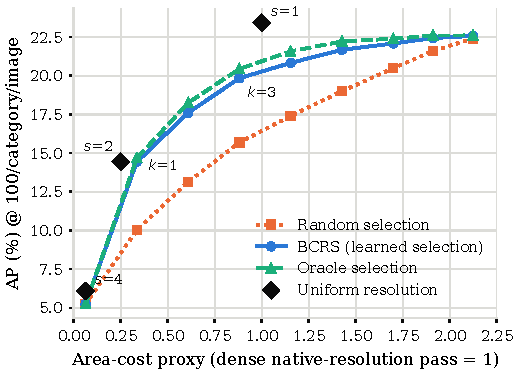
\includegraphics[width=\columnwidth]{figures/curve.pdf}\\[2pt]
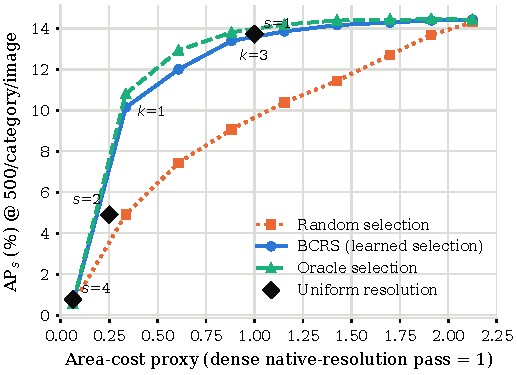
\includegraphics[width=\columnwidth]{figures/curve_aps.pdf}
\caption{Corrected v3 seed-0 AP and small-object AP against the area-cost proxy of Eq.~\eqref{eq:proxy}, showing $k=0,\ldots,8$ (full-sweep AUC additionally uses $k=9,\ldots,15$). Evaluator caps per category per image: AP 100, small-object AP 500. Selection curves share detector weights and fusion; diamonds are separately trained uniform-resolution models. Oracle denotes a missed-object-count ranking, not a guaranteed AP bound.}
\label{fig:curve}
\end{figure}
At three tiles, learned selection obtains 19.84 AP and random selection 15.68 AP, a 4.16-point improvement at the same tile count. The oracle reaches 20.44 AP. Over $k=0,\ldots,15$, with proxy cost from 0.0625 to 2.1906, unnormalized trapezoidal AP-versus-proxy-cost areas are 0.405, 0.347, and 0.414 for learned, random, and oracle rankings, respectively (AP expressed as a fraction for integration). Learned selection recovers approximately 87\% of the oracle-minus-random area difference. This statistic measures ranking quality within the tile system, not efficiency relative to dense inference.
Table~\ref{tab:budget-breakdown} separates the three-tile comparison by metric. Learned selection raises AP$_s$ by 4.3 points and AP$_m$ by 3.3 points over random selection; AP$_l$ is 39.2 for both after rounding.

The dense comparison is less favorable. Three-tile BCRS reaches 19.8 AP and 13.4 AP$_s$ at proxy cost 0.88, below dense native inference at 23.4 and 13.7. One tile reaches 14.4 AP at cost 0.34, approximately the half-resolution model's AP at cost 0.25, although its small-object AP is higher (10.1 versus 4.9). With zero tiles, BCRS reaches 5.2 AP, below the quarter-resolution baseline's 6.1. At exhaustive selection ($k=15$, with tile counts capped per frame), seed-0 BCRS reaches 22.6 AP at proxy cost about 2.19, still below the dense baseline. These points do not establish a general advantage over uniform inference.

The frozen two-pass configuration reaches 19.83 AP at three tiles, almost identical to the joint model's 19.84. Joint training increases small-object AP there from 12.89 to 13.39, but whole-image inference with the joint weights falls to 22.83 AP from the native initialization's 23.40 in the frozen sweep's whole-image branch (23.43 in standalone evaluation). Exhaustive selection changes from 22.55 to 22.59 AP. The corrected results therefore do not support the earlier claim that joint training produces a large overall tile-accuracy gain.

\subsection{Tiling and coordinate precision}
\label{sec:fusion}
With frozen v3 detectors, exhaustive tiling gives 22.55 AP versus 23.40 for the whole-image branch of the same sweep. AP$_s$ is 13.61 versus 13.70, and AP$_l$ is 45.48 versus 47.96. Tiling does not reproduce whole-image context: crops can truncate objects, alter padding and context, and change candidate filtering and fusion. Therefore equality is not an expected invariant, even with unchanged detector weights.

\begin{table}[t]
\caption{Same-checkpoint numerical diagnostic (v2 weights, no retraining). The correction changes decoding and score post-processing to float32; it does not change backbone precision. Raw sources: \texttt{fp32eval\_uniform} (baseline, both modes) and \texttt{p3\_sweep\_joint\_v2} / \texttt{p3\_sweep\_joint\_v2\_fp32} (joint). AP in percent, with 100 detections per category per image.}
\label{tab:precision}
\centering
\begin{tabular}{p{0.57\columnwidth}rr}
\toprule
Inference & Legacy & Corrected \\
\midrule
Native baseline, standalone evaluation & 15.88 & 19.09 \\
Joint detector, whole image & 14.15 & 22.42 \\
Joint detector, learned $k=3$ & 19.60 & 19.76 \\
\bottomrule
\end{tabular}
\end{table}
The same-checkpoint comparison in Table~\ref{tab:precision} isolates the numerical post-processing change from retraining. Whole-image AP with the joint detector increases by 8.27 points, but its three-tile AP increases by only 0.16. The apparent advantage of three tiles over the same detector on whole images changes from $+5.45$ to $-2.66$ AP. The standalone native baseline also increases by 3.22 AP from the unrounded values; legacy mode reproduces the archived legacy evaluation. This is evidence of an asymmetric numerical confound, not a benefit of new training. It does not isolate coordinate precision from score precision, since both are corrected together.

The large unexplained tiling advantage in the earlier draft is absent after corrected training and decoding. Low-precision coordinates were a confound in that comparison. We do not attribute every remaining difference to one mechanism: separate changes to context, clipping, and candidate caps would require controlled experiments. The size-aware fusion rule remains fixed across current selection comparisons; its independent contribution is not measured by those comparisons.

\subsection{Ablations}
\label{sec:ablations}
\begin{table*}[t]
\caption{Ablations on VisDrone-DET val. AP (\%) at $k$ selected tiles, AP$_s$ and selection recall (\%) at $k{=}3$, and area under the AP-versus-cost curve over the full sweep (cost 0.06 to 2.19 in units of one dense native pass). Evaluator caps per category per image: AP 100, AP$_s$ 500. Recall is the mean per-image unique-owner recall over images with misses. Rows (ii)--(iv) are separate 12-epoch joint trainings from the same initialization; row (i) re-evaluates the full model with the budget input held at $b{=}3/20$ for every $k$. One training run (seed 0) per row; at the displayed budgets, the largest AP difference from the full model is 0.6 points. Corrected v3 generation.}
\label{tab:ablation}
\centering
\begin{tabular}{lcccccccc}
\toprule
Variant & $k{=}1$ & $k{=}2$ & $k{=}3$ & $k{=}4$ & $k{=}6$ & AP$_s$@3 & Rec@3 & AUC \\
\midrule
Full model (perturbed top-$k$, self-derived targets, FiLM) & 14.4 & 17.6 & 19.8 & 20.8 & 22.1 & 13.4 & 75.8 & 0.405 \\
(i) budget input fixed at evaluation & 14.3 & 17.6 & 19.8 & 20.8 & 22.2 & 13.4 & 75.8 & 0.405 \\
(ii) object-count targets, no refinement & 14.6 & 17.7 & 20.2 & 21.2 & 22.4 & 13.6 & 77.5 & 0.410 \\
(iii) Gumbel-softmax surrogate & 15.0 & 18.0 & 20.3 & 21.4 & 22.3 & 13.6 & 77.6 & 0.413 \\
(iv) no gradient through selection & 14.6 & 17.7 & 20.1 & 21.2 & 22.4 & 13.6 & 77.5 & 0.409 \\
\bottomrule
\end{tabular}
\end{table*}

The fixed-input v3 ablation holds the scorer input at $b=3/20$ while changing the hard tile cap. At the displayed budgets, the maximum AP change is approximately 0.13 points, and the full-sweep AUC is approximately 0.405 in both cases. At $k=3$ the inputs are identical by construction. This supports a small effect of changing the conditioning input for this trained model. It does not test training without FiLM, nor establish equivalence across seeds.

The three retraining ablations use the corrected v3 protocol and one seed each. Object-count targets count all ground-truth objects and disable recovery refinement; this combined target-construction change reaches 20.24 AP at three tiles, compared with 19.84 for the full model; the largest absolute difference over the sweep is 0.40 points. A straight-through Gumbel-softmax surrogate, with the same hard forward top-$k$, reaches 20.27 AP at three tiles and differs by up to 0.56 points, at four tiles. Removing the selection gradient, while retaining direct scorer supervision, reaches 20.09 AP at three tiles and differs by up to 0.33 points, at four tiles. Full-sweep AUCs are 0.410, 0.413, and 0.409, respectively, versus 0.405 for the full model.

The Gumbel ablation is a local straight-through subset surrogate inspired by~\cite{jang2017gumbel}, not a direct reproduction of its categorical estimator. Starting with $a_0=\mathbf s$, each of $k$ steps draws fresh Gumbel noise $\boldsymbol\gamma_j$, computes $p_j=\operatorname{softmax}((a_j+\boldsymbol\gamma_j)/0.5)$, and updates $a_{j+1}=a_j+\log(1-\min(\operatorname{sg}[p_j],1-10^{-6}))$. The sum of the $p_j$ supplies the backward surrogate; the forward result remains deterministic hard top-$k$. This finite-temperature update reduces probability mass rather than guaranteeing sampling without replacement.

At three tiles, these improvements over seed 0 are 0.40, 0.43, and 0.25 AP points, exceeding the full model's observed three-seed range of approximately 0.16 points. They must not be summarized as identical results or as differences entirely explained by the measured full-model spread. However, each ablation has only one training run: the full-model spread is not an estimate of each variant's variance and does not establish statistical significance. The results provide no evidence that miss-derived targets or a selection gradient are necessary for this setting, and motivate a simpler directly supervised selector. They do not test removing several mechanisms together, nor show that the alternatives consistently improve AP across training seeds. None changes the broader conclusion that dense native inference has higher overall AP.

\subsection{Variation across joint-training seeds}
\label{sec:seeds}
\begin{table}[t]
\caption{Seed variation of the jointly trained model: AP (\%) with learned selection at $k$ tiles, and whole-image inference with the same detector, for three joint trainings that differ only in the seed. Mean $\pm$ sample standard deviation over the three runs. AP uses 100 detections per category per image. Corrected v3 generation.}
\label{tab:seeds}
\centering
\begin{tabular}{lccccc}
\toprule
Inference & Cost & Seed 0 & Seed 1 & Seed 2 & Mean \\
\midrule
whole image & 1.00 & 22.8 & 22.8 & 22.8 & 22.8 $\pm$ 0.01 \\
$k{=}1$ & 0.34 & 14.4 & 14.5 & 14.4 & 14.4 $\pm$ 0.04 \\
$k{=}2$ & 0.61 & 17.6 & 17.9 & 17.7 & 17.7 $\pm$ 0.14 \\
$k{=}3$ & 0.88 & 19.8 & 20.0 & 19.9 & 19.9 $\pm$ 0.08 \\
$k{=}4$ & 1.15 & 20.8 & 21.1 & 21.0 & 21.0 $\pm$ 0.15 \\
$k{=}6$ & 1.70 & 22.1 & 22.3 & 22.2 & 22.2 $\pm$ 0.11 \\
$k{=}8$ & 2.12 & 22.6 & 22.8 & 22.7 & 22.7 $\pm$ 0.11 \\
\bottomrule
\end{tabular}
\end{table}

At three tiles, AP is 19.84, 20.00, and 19.93 across seeds 0, 1, and 2, giving a mean of 19.9 and sample standard deviation of 0.08 AP points (Table~\ref{tab:seeds}). At one tile the mean is 14.4 with standard deviation 0.04. These are descriptive statistics over three joint trainings from a shared initialization, not confidence intervals. They do not replace replicated ablations or independent baseline retraining.
Figure~\ref{fig:seed-variation} places the seed spread beside the two single-run dense controls at each reported budget. The three-seed mean remains below both controls for overall AP.
\begin{figure*}[t]
\centering
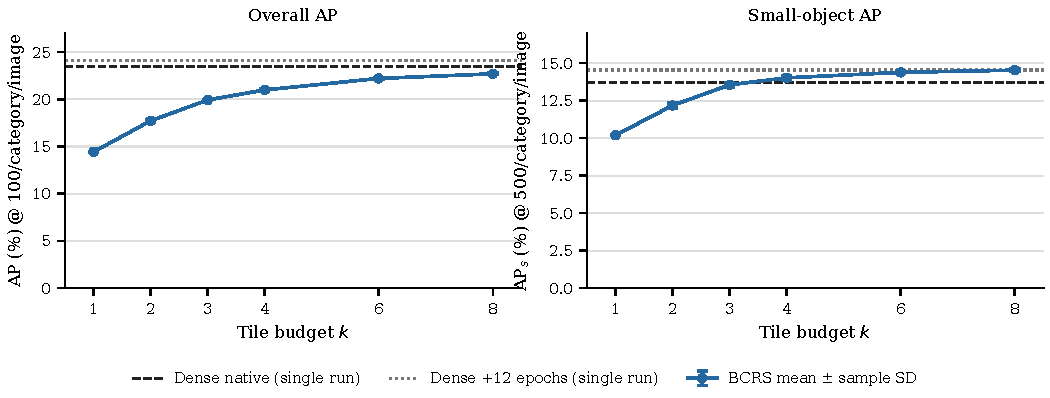
\includegraphics[width=\textwidth]{figures/seed_variation.pdf}
\caption{Mean AP and AP$_s$ at $k=1,2,3,4,6,8$ for three joint-training seeds. Error bars show sample standard deviation across seeds. They do not estimate confidence intervals. Dashed and dotted lines show the separately trained dense baseline and its 12-epoch continuation. Each reference uses one run. All three joint runs share a pretrained initialization. AP uses 100 detections per category per image; AP$_s$ uses 500. Sources: \texttt{p3\_sweep\_joint\_v3}, \texttt{p3\_sweep\_joint\_v3\_seed1}, \texttt{p3\_sweep\_joint\_v3\_seed2}, and \texttt{v3eval\_uniform}.}
\label{fig:seed-variation}
\end{figure*}

\subsection{Measured latency}
\label{sec:latency}
\begingroup
\setlength{\tabcolsep}{5pt}
\begin{table}[t]
\caption{Median timings (ms/frame) on VisDrone-DET val subsets. All modes use joint detector weights, not the separately trained dense accuracy baselines. GPU: NVIDIA A100-PCIE-40GB, bf16, shared. b1: median of per-image component sums, excluding top-$k$, initial host-to-device transfer and loading (100 timed images); scoring includes device-to-host transfer. b8: median batch time divided by eight (nine timed batches); fine tiles are chunked at 32. CPU: AMD EPYC 7502 32-Core Processor, fp32, 40 timed images. Cost is a pixel-area proxy, not measured operations. See Section~\ref{sec:latency} for scope and mean-versus-median differences (source: \texttt{latency\_v3}). Corrected v3 generation.}
\label{tab:latency}
\centering
\begin{tabular}{lccccc}
\toprule
Mode & Cost & GPU b1 & GPU b8 & CPU 4 thr. & CPU 16 thr. \\
\midrule
Dense, $s{=}4$ & 0.06 & 19.3 & 6.8 & 108.9 & 57.7 \\
Dense, $s{=}2$ & 0.25 & 19.2 & 6.2 & 278.5 & 118.7 \\
Dense, $s{=}1$ & 1.00 & 19.3 & 12.7 & 1004.1 & 389.1 \\
BCRS, $k{=}1$ & 0.34 & 42.7 & 16.2 & 386.1 & 173.6 \\
BCRS, $k{=}2$ & 0.61 & 47.8 & 24.5 & 628.4 & 256.3 \\
BCRS, $k{=}3$ & 0.88 & 53.1 & 32.3 & 902.1 & 358.3 \\
BCRS, $k{=}4$ & 1.15 & 60.5 & 38.4 & 1143.8 & 462.0 \\
BCRS, $k{=}6$ & 1.70 & 73.8 & 55.0 & 1706.3 & 682.1 \\
\bottomrule
\end{tabular}
\end{table}

\begin{table}[t]
\caption{Batch-one timing spread for the joint detector on VisDrone-DET val. Values are milliseconds per frame from per-image component sums. Each mode uses 100 timed images on a shared A100. The p95 describes this sample and is not a deadline guarantee. Source: \texttt{latency\_v3/gpu\_b1.json}.}
\label{tab:latency_spread}
\centering
\begin{tabular}{lccc}
\toprule
Mode & Median & Mean & p95 \\
\midrule
Dense native & 19.3 & 22.3 & 37.4 \\
BCRS, $k{=}1$ & 42.7 & 45.8 & 61.2 \\
BCRS, $k{=}3$ & 53.1 & 58.1 & 81.1 \\
BCRS, $k{=}6$ & 73.8 & 76.8 & 103.5 \\
\bottomrule
\end{tabular}
\end{table}

\endgroup
Table~\ref{tab:latency} reports the archived v3 timings. All modes use the joint detector; its whole-image AP is 22.83, not the separately trained baseline's 23.43. On the A100 at batch one, three-tile BCRS takes 53.1\,ms per frame versus 19.3\,ms for native whole-image inference with those same joint weights, about 2.74 times as long using unrounded timings. Even one tile takes 42.7\,ms. With batches of eight, three-tile throughput corresponds to 32.3\,ms per frame versus 12.7\,ms for dense native processing. The batch-eight protocol also shows a GPU disadvantage; differences in sampled images and timing procedure prevent attributing the change solely to batching.
Figure~\ref{fig:latency-cost} shows that a lower area-cost proxy does not ensure a lower measured GPU time in either protocol. Table~\ref{tab:latency_spread} reports the batch-one timing spread. The p95 is 81.1\,ms at $k=3$ and 37.4\,ms for dense native inference. Both percentiles summarize 100 images on a shared A100 and do not define deadline bounds.
\begin{figure*}[t]
\centering
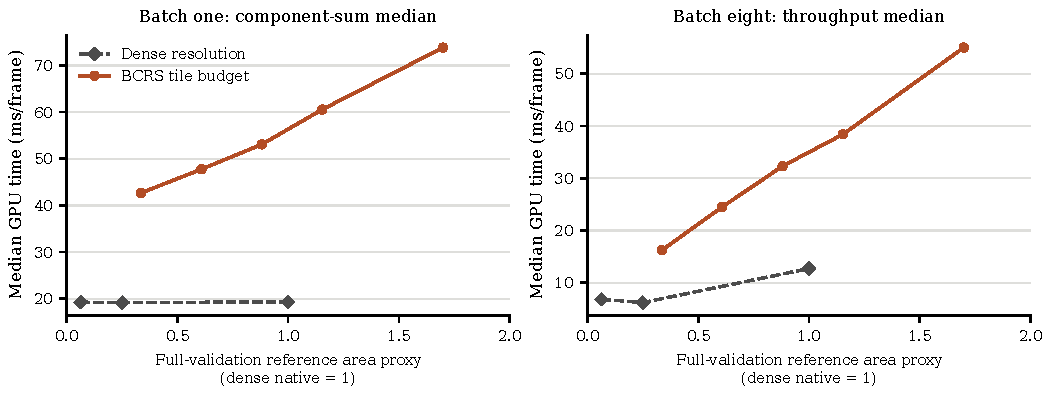
\includegraphics[width=\textwidth]{figures/latency_cost.pdf}
\caption{Median GPU time against the full-validation reference area-cost proxy. All modes use the same joint detector weights. Batch one reports per-image component-sum medians over 100 images. Batch eight reports median batch time per frame over nine batches of $1360\times765$ frames. Its $k=3$ per-frame proxy is 0.818; the plot uses the full-validation reference proxy in both panels. The panels use different timing protocols on a shared A100. Sources: \texttt{latency\_v3/gpu\_b1.json}, \texttt{latency\_v3/gpu\_throughput\_b8.json}, and \texttt{p3\_sweep\_joint\_v3}.}
\label{fig:latency-cost}
\end{figure*}

Batch-one BCRS timing is the median of per-image sums of separately synchronized coarse, scorer, fine, and fusion regions, not the sum of component medians. Scoring includes copying scores to CPU. The sums exclude image decoding, initial host-to-device transfer, grid and budget construction, and top-$k$ sorting. GPU medians use 100 timed images after ten warm-ups; CPU medians use 40 after three warm-ups, from seed-0 shuffled validation subsets. Batch-eight timing uses $1360\times765$ images: twelve batches are loaded, three discarded for warm-up, leaving nine timed batches (72 frames). It reports the median batch duration divided by eight, with fine tiles processed in chunks of at most 32. cuDNN benchmarking is disabled for component timings and enabled for the throughput test.

On the EPYC CPU, three tiles take 902.1\,ms with four threads versus 1004.1\,ms for dense native inference, or 358.3 versus 389.1\,ms with 16 threads. These are median reductions only. Mean CPU time reverses the three-tile comparison: 901.2 versus 878.6\,ms with four threads, and 359.7 versus 344.0\,ms with sixteen threads. Thus the data do not establish a reduction in average CPU processing time. CPU inference uses float32 backbone operations, whereas the reported AP uses bf16; CPU accuracy was not measured separately. The A100 was shared; these measurements are not isolated-device service-level guarantees. Resize placement, post-processing, image-size batching, and other-user load must be retained when reproducing them.

\section{Limitations}
\label{sec:limitations}
All accuracy experiments use one dataset and its validation split, with a relatively small ResNet-18 FCOS detector. There is no held-out test result, stronger-backbone replication, or controlled comparison with a published selective detector. Baselines and initialization stages are single runs; three joint-training seeds cover only one source of variation.

The area-cost proxy is not a hardware-independent speed claim. It omits overhead and uses the split's mean area. A deployment that requires a deadline must calibrate and validate latency on its own hardware; a fixed tile count is insufficient. The current GPU results favor whole-image inference with joint weights; the CPU comparison depends on whether means or medians are used. No energy measurements are available.

Selection targets and the oracle count missed objects rather than their marginal contribution to final AP. Overlapping tiles and fusion create interactions that this count does not model. A different scorer objective might help, but the current experiments do not establish that it would. The retraining ablations are single runs. Their favorable point estimates warrant replication and a combined simplification test before claiming a consistently better training recipe.

Validation is used both to choose checkpoints and to report accuracy, so these results are not held-out generalization estimates. The archives record source commits and checkpoint paths but not checkpoint hashes or exact server dependency versions. In particular, the mixed-cap AP definition follows the inspected standard COCO summarizer; the historical server copy is not archived. The cited evaluator is pinned for inspection, not asserted to be the server version. Regression tests verify the cap behavior in a fresh environment without re-evaluating archived checkpoints. Aggregate latency records do not retain per-image samples, limiting uncertainty analysis.

\section{Conclusion}
BCRS provides an inference-time tile cap and a learned ranking that improves substantially over random selection at the same tile budget. Across three joint-training seeds it reaches 19.9 AP at three tiles. Corrected float32 decoding changes the broader interpretation: dense native inference reaches 23.4 AP, a matched-epochs dense control reaches 24.1, and measured A100 whole-image inference with joint weights is faster than the tiled path. The supported contribution is an analysis of selective inference and its evaluation constraints, not a demonstrated general efficiency improvement over dense detection. Coordinate precision, comparison controls, actual image geometry, and measured runtime are necessary parts of that analysis. Corrected ablation point estimates favor object-count targets and show that direct supervision can train the scorer without a selection gradient in this setting. These single-run findings motivate replicated simplification experiments rather than a claim of statistical equivalence or universal superiority.

\IEEEtriggeratref{27}
\bibliographystyle{IEEEtran}
\bibliography{references}
\end{document}
